\chapter{PCB 3.0 改进设计和测试}
\label{cha:PCB-v3}

\section{待改进问题}

三路驱动丝印编号

电池插头+-反向,以丝印标注

芯片周围留出clearance,方便拖焊。摆放可以考虑45度角摆放,方便密集的布线。

最好改成单面有贴片元件的形式,方便SMT或者制作钢网涂锡膏。

选用没有ThermalVias的芯片封装,否则容易焊锡粘到了ThermalVias上引起不平整。(但是没有不含ThermalPad的封装)

留出STEP和DIR测试/备用引脚,以便板上有一两片DRV8825无法正常使用可以外接模块。

12V和5V供电太细了,要注意供电可靠性。

扩大PCB面积,从100mm到120mm直径圆内接正六边形。

Reset按钮封装不对。Reset电路中R22/D1,RESET BUTTON/C13不是必须的,可以画,可以不焊。

!!!发现CH340C的TX接到了Mega的TX上,RX接到了Mega的RX上,所以烧录Arduino时出现错误:

\begin{tcolorbox}
    avrdude: stk500v2\_ReceiveMessage(): timeout \\
    avrdude: stk500v2\_getsync(): timeout communicating with programmer
\end{tcolorbox}


\section{外形}

小车外轮廓为120mm圆内接正六边形,为了尽可能放到单面上,设计成120mm圆内接正六边形,加上40mm半径处3mm直径的M3螺丝定位孔,注意孔位置在边上而不是角上。注意Fusion360导出草图的操作是直接右键草图另存为DXF!

\section{原理图更改}

在这个版本,删去了一些演示中暂时用不到的模块:

\begin{itemize}
    \item RGB-LED阵列
    \item 下视相机模块
    \item 控制步进的拨码开关
    \item Reset按钮和电容/CD1206二极管
\end{itemize}

同时将XT30的正负极反向,修正了封装和实际不对应的问题。

TX0和RX0倒序,纠正了错误。

原理图如图~\ref{fig:MisakaPCBv3-sch}。

\begin{figure}[htbp]
    \centering
    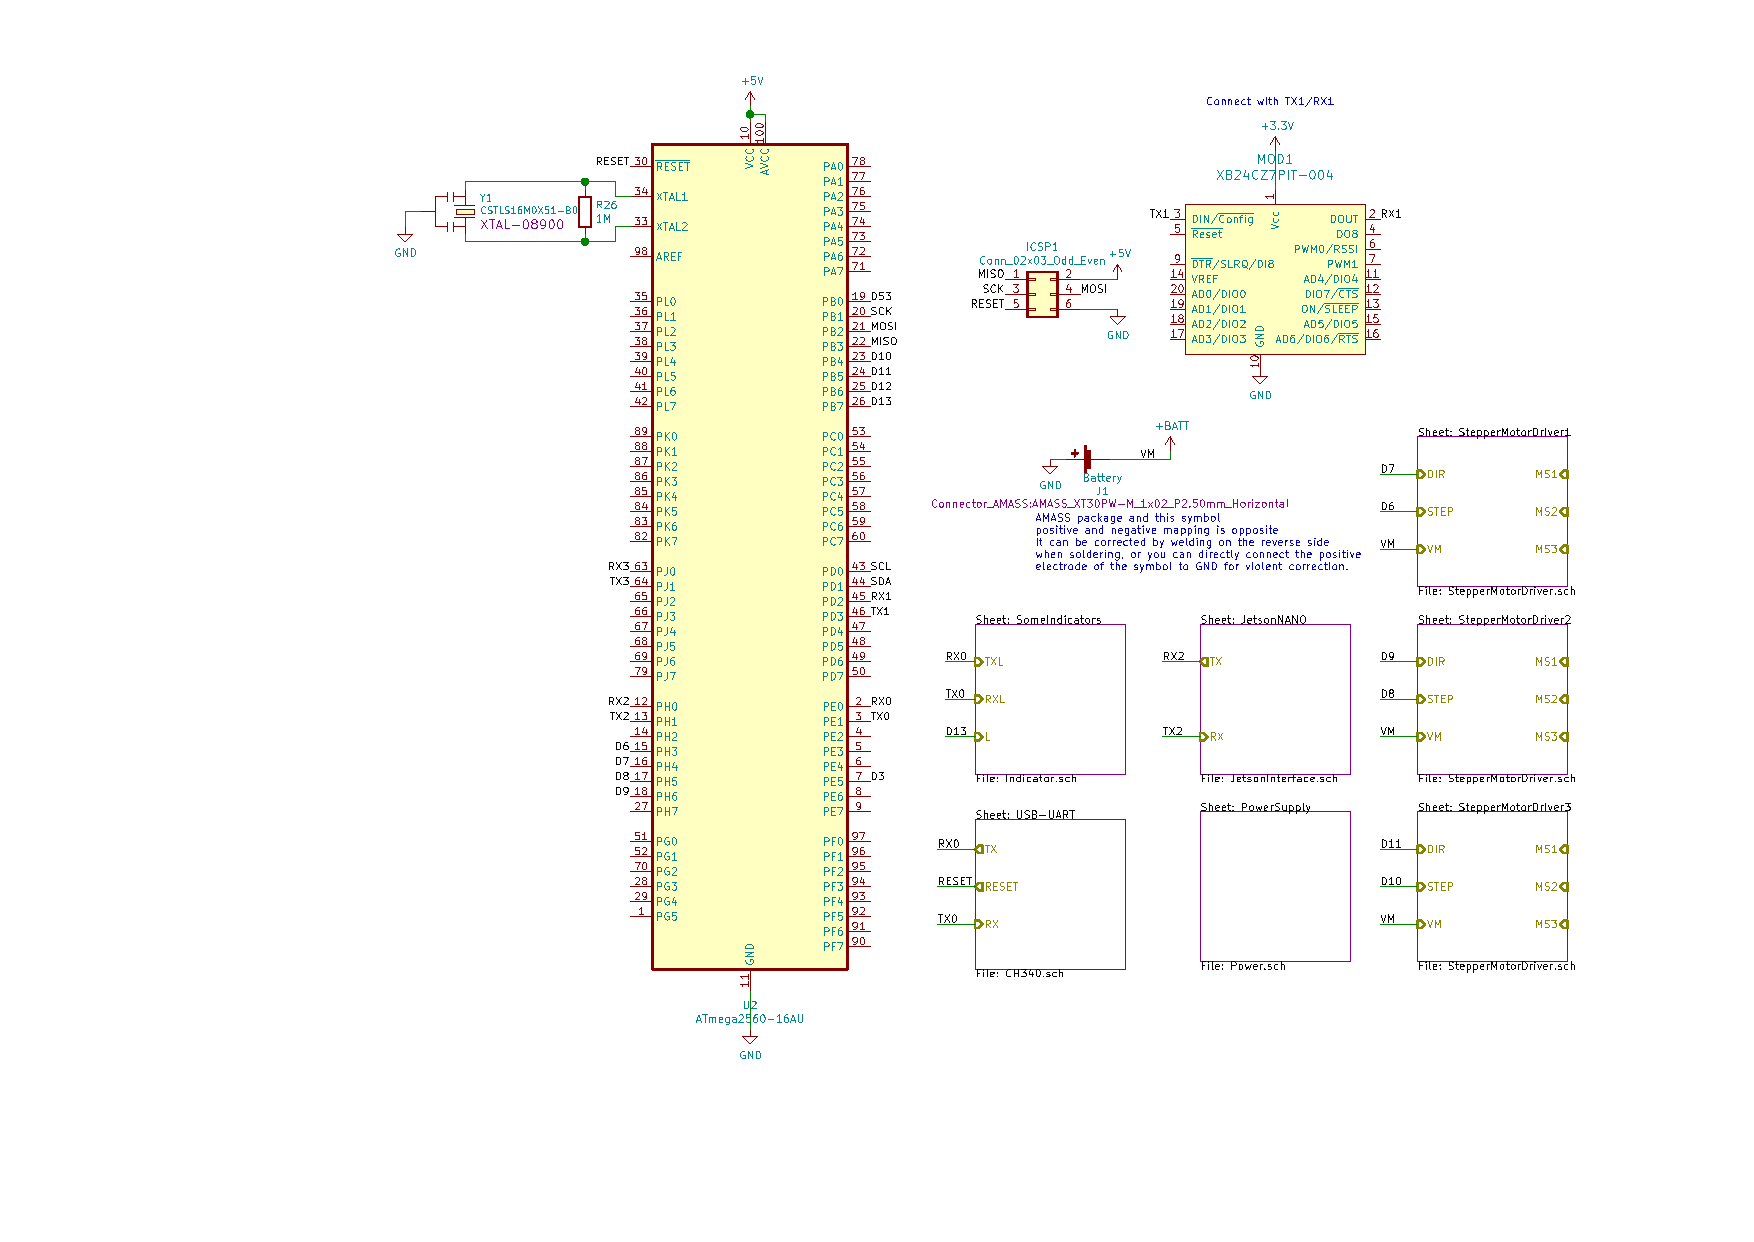
\includegraphics[width=\columnwidth]{MisakaPCBv3-1.pdf}
    \caption{PCBv3原理图}
    \label{fig:MisakaPCBv3-sch}
\end{figure}

\section{PCB绘制}

将MCU倾斜45度,方便布线。

加粗12V和5V干线至1mm宽。

三个电机驱动模块统一布局布线,使其具有相似性,并变得整齐。

考虑到走线问题,同一功能的信号线组并在一起。

% 布线之后的PCB详见附录~\ref{sec:PCB}。

布线之后的PCB(未显示铺铜)如图~\ref{fig:MisakaPCBv3-1}、~\ref{fig:MisakaPCBv3}。

\begin{figure}[htbp]
    \centering
    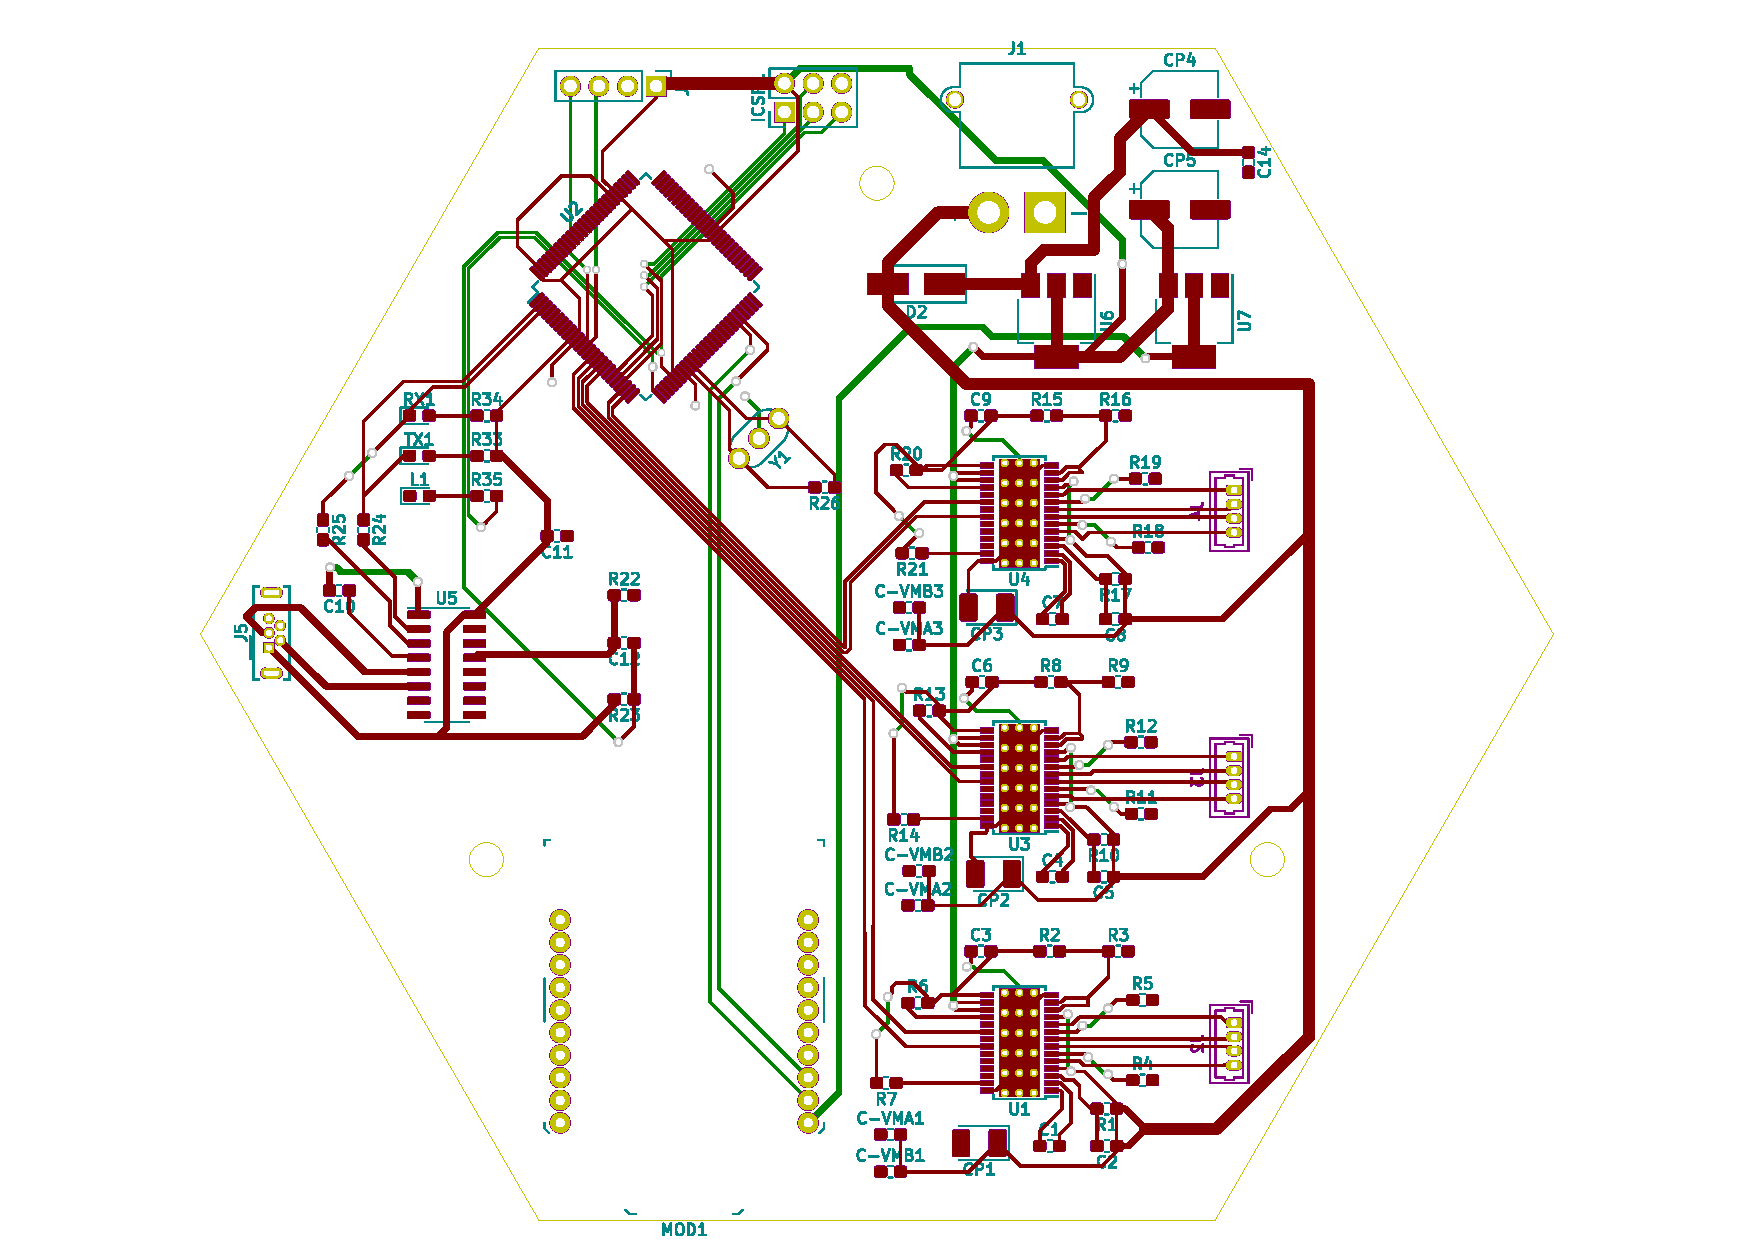
\includegraphics[width=\columnwidth]{MisakaPCBv3-2.pdf}
    \caption{PCBv3布线}
    \label{fig:MisakaPCBv3}
\end{figure}

\begin{figure}[htbp]
    \centering
    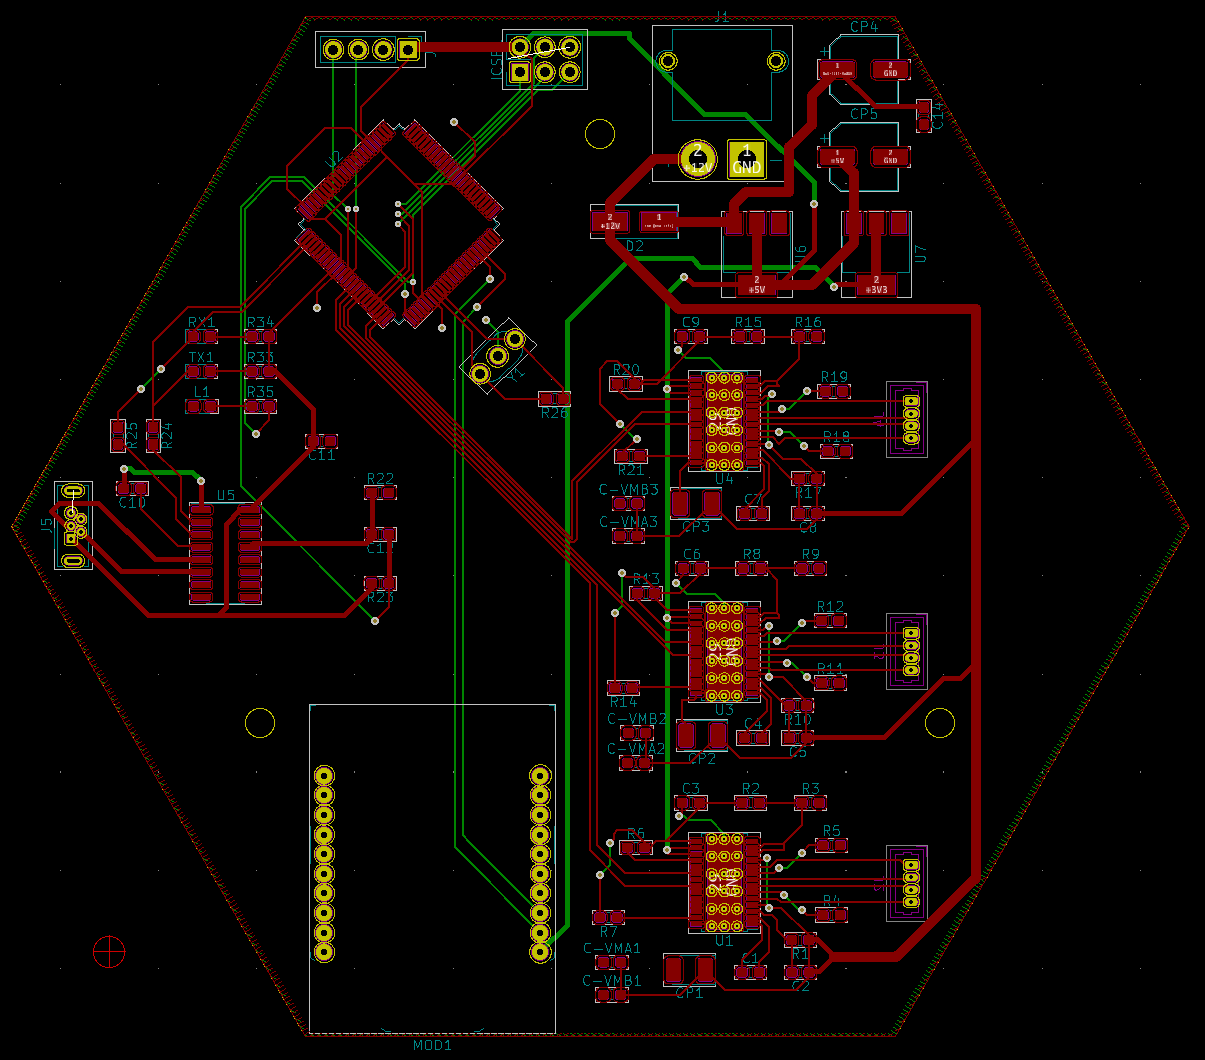
\includegraphics[width=\columnwidth]{MisakaPCBv3-1.png}
    \caption{PCBv3布线之后的PCB}
    \label{fig:MisakaPCBv3-1}
\end{figure}

\section{三维渲染图}

使用光线追踪技术对PCB模型进行渲染得到正面的渲染图如图~\ref{fig:MisakaPCBv3-2}、~\ref{fig:MisakaPCBv3-3}。

\begin{figure}[htbp]
    \centering
    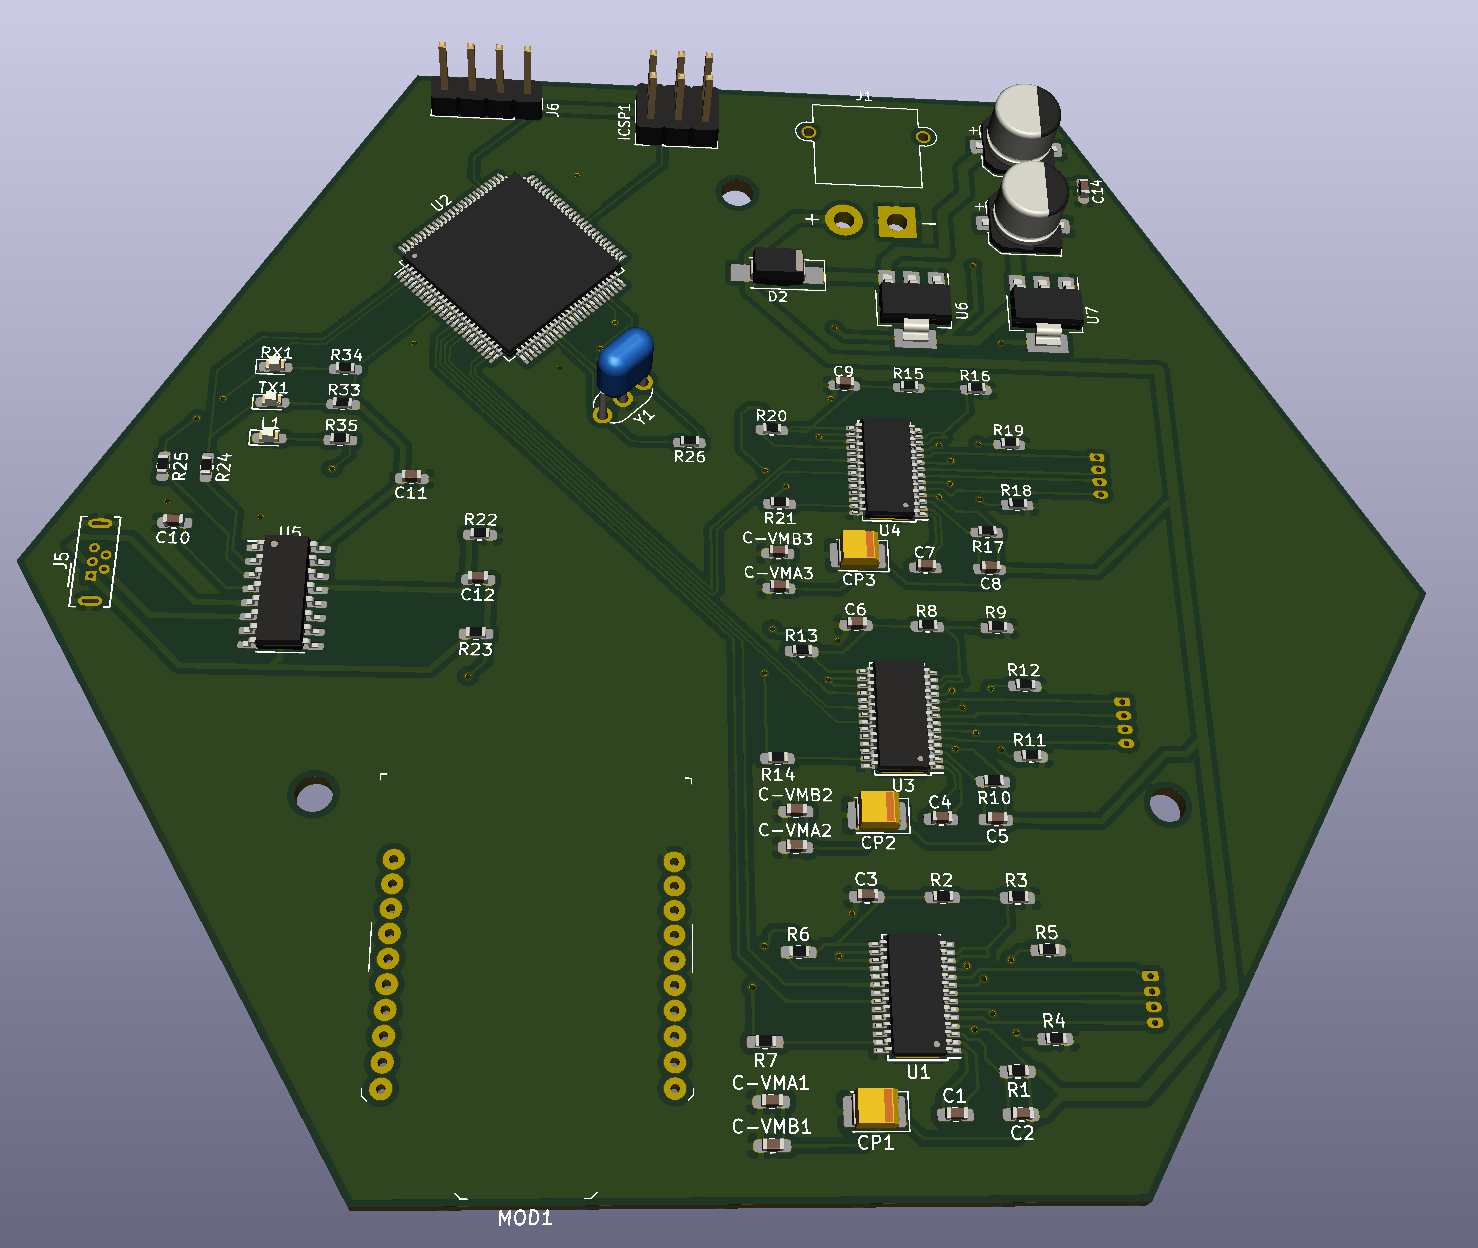
\includegraphics[width=\columnwidth]{MisakaPCBv3-2.png}
    \caption{正面渲染图}
    \label{fig:MisakaPCBv3-2}
\end{figure}

\begin{figure}[htbp]
    \centering
    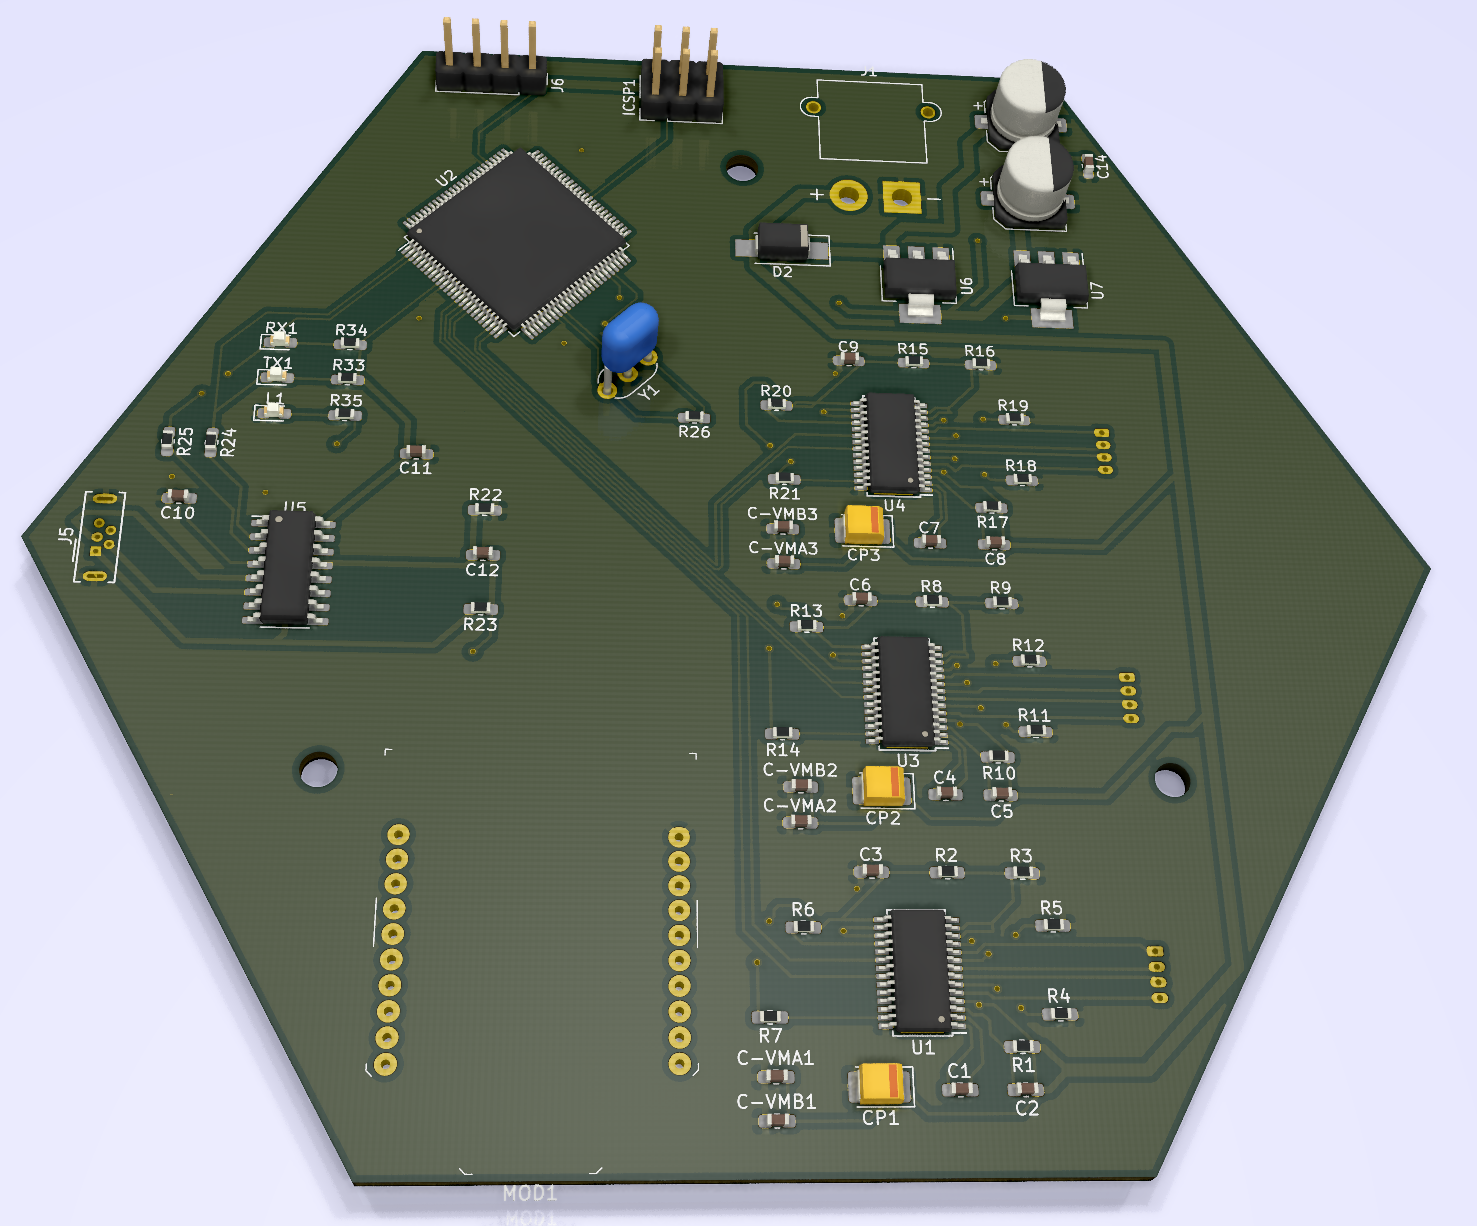
\includegraphics[width=\columnwidth]{MisakaPCBv3-3.png}
    \caption{光追渲染图}
    \label{fig:MisakaPCBv3-3}
\end{figure}

\section{其他问题}

应当加一个ON LED作为电源指示灯。

没有Reset很麻烦,特别是一开始调试的时候,需要按Reset重置代码。考虑加一个Reset按钮到GND和一个22pF电容并连。
